\documentclass[titlepage, fleqn, a4paper, 12pt, twoside]{article}
\usepackage{geometry}
\usepackage{exsheets} %question and solution environments
\usepackage{amsmath, amssymb, amsthm} %standard AMS packages
\usepackage{esint} %integral signs
\usepackage{marginnote} %marginnotes
\usepackage{gensymb} %miscellaneous symbols
\usepackage{commath} %differential symbols
\usepackage{xcolor} %colours
\usepackage{cancel} %cancelling terms
\usepackage[free-standing-units]{siunitx} %formatting units
\usepackage{tikz, pgfplots} %diagrams
	\usetikzlibrary{calc, hobby, patterns, intersections, angles, quotes, spy}
\usepackage{graphicx} %inserting graphics
\usepackage{epstopdf} %converting and inserting eps graphics
\usepackage{hyperref} %hyperlinks
\usepackage{datetime} %date and time
\usepackage{enumerate, enumitem} %numbered lists
\usepackage{float} %inserting floats
\usepackage{microtype} %micro-typography
\usepackage{todonotes}
\usepackage{booktabs}
\usepackage{xspace}

\newcommand\numberthis{\addtocounter{equation}{1}\tag{\theequation}} %adds numbers to specific equations in non-numbered list of equations

\theoremstyle{definition}
\newtheorem{example}{Example}
\newtheorem{definition}{Definition}

\theoremstyle{theorem}
\newtheorem{theorem}{Theorem}
\newtheorem{law}{Law}
\newtheorem{axiom}{Axiom}

\makeatletter
\@addtoreset{section}{part} %resets section numbers in new part
\makeatother

\newcommand\blfootnote[1]{%
	\begingroup
	\renewcommand\thefootnote{}\footnote{#1}%
	\addtocounter{footnote}{-1}%
	\endgroup
}

\renewcommand{\marginfont}{\scriptsize \color{blue}}

\renewcommand{\tilde}{\widetilde}

\DeclareMathOperator{\comp}{\textsc{c}}

\DeclareMathOperator{\prob}{\mathrm{P}}

\DeclareMathOperator{\expct}{\mathrm{E}}

\DeclareMathOperator{\var}{\mathrm{V}}

\DeclareMathOperator{\sd}{\mathrm{\sigma}}

\DeclareMathOperator{\cdf}{\mathrm{cdf}}

\DeclareMathOperator{\bin}{\mathrm{Bin}}

\newcommand*{\perm}[2]{{}^{#1}\mathrm{P}_{#2}}%
\newcommand*{\comb}[2]{{}^{#1}\mathrm{C}_{#2}}%

\newcommand{\A}{\text{Alice}\xspace}
\newcommand{\B}{\text{Bob}\xspace}
\newcommand{\C}{\text{Charlie}\xspace}
\newcommand{\D}{\text{David}\xspace}
\newcommand{\E}{\text{Eve}\xspace}
\newcommand{\F}{\text{Frank}\xspace}

\SetupExSheets{solution/print = true} %prints all solutions by default

\newtoggle{paper}

\toggletrue{paper}

\iftoggle{paper}{

}{
	\usepackage{setspace}
	\doublespacing
}

%opening
\title{Introduction to Probability and Statistics}
\author{Aakash Jog}
\date{2015-16}

\begin{document}

\pagenumbering{roman}
\begin{titlepage}
\newgeometry{margin=0cm}
\maketitle
\end{titlepage}
\restoregeometry
%\setlength{\mathindent}{0pt}

\blfootnote
{	
	\begin{figure}[H]
		
\includegraphics[height = 12pt]{cc.pdf}
		
\includegraphics[height = 12pt]{by.pdf}
		
\includegraphics[height = 12pt]{nc.pdf}
		
\includegraphics[height = 12pt]{sa.pdf}
	\end{figure}
	This work is licensed under the Creative Commons Attribution-NonCommercial-ShareAlike 4.0 International License. To view a copy of this license, visit \url{http://creativecommons.org/licenses/by-nc-sa/4.0/}.
} %CC-BY-NC-SA license

\tableofcontents

\clearpage
\section{Lecturer Information}

\textbf{Dr. Galit Ashkenazi-Golan}\\
~\\
E-mail: \href{mailto:galit.ashkenazi@gmail.com}{galit.ashkenazi@gmail.com}\\

\section{Instructor Information}

\textbf{Liran Mendel}\\
~\\
E-mail: \href{mailto:liran.mendel@gmail.com}{liran.mendel@gmail.com}\\

\section{Recommended Reading}

\begin{enumerate}
	\item Sheldon M. Ross: A First Course in Probability Pearson Prenticce Hall, 8th Edition, 2010.
	\item Bertsekas, Dimitri P. and Tsitsikis, John N., Introduction to Probability. Athena Science, 2nd editions, 2008.
	\item Montgomery, D.C and Runger, G.C. and Hubele, N.F. Engineering Statistics. Wiley \& Sons, NY, 4th Edition, 2007.
\end{enumerate}

\clearpage
\pagenumbering{arabic}

\part{Basics of Probability}

\section{Terminology}

\begin{definition}[Experiment]
	A situation with uncertain results is called an experiment.
\end{definition}

\begin{definition}[Sample space]
	The set of all possible outcomes of an experiment is called the sample space.
	It is denoted by $\Omega$ or $S$.
\end{definition}

\begin{definition}[Event]
	Any subset $A$ of the sample space is called an event.
\end{definition}

\begin{definition}[Intersection of sets]
	Let $A$ and $B$ be two events of sample space $\Omega$.
	The set of all outcomes that are both in $A$ and $B$ is called the intersection of $A$ and $B$.
	It is denoted by $A \cap B$.
\end{definition}

\begin{definition}[Union of sets]
	Let $A$ and $B$ be two events of sample space $\Omega$.
	The set of all outcomes that are in either of $A$ and $B$ is called the union of $A$ and $B$.
	It is denoted by $A \cup B$.
\end{definition}

\begin{definition}[Complement of set]
	Let $A$ be an event of sample space $\Omega$.
	The set of all outcomes that are not in $A$, but are in $\Omega$ is called the complement of $A$.
	It is denoted by $\overline{A}$ or $A^{\comp}$.
\end{definition}

\begin{definition}[Mutually exclusive events]
	Two events $A$ and $B$ are said to be mutually exclusive, if
	\begin{align*}
		A \cap B & = \emptyset
	\end{align*}
\end{definition}

\section{Basic Laws}

\begin{law}[Commutative Laws]
	\begin{align*}
		A \cup B & = B \cup A \\
		A \cap B & = B \cap A
	\end{align*}
\end{law}

\begin{law}[Associative Laws]
	\begin{align*}
		(A \cup B) \cup C & = A \cup (B \cup C) \\
		(A \cap B) \cap C & = A \cap (B \cap C)
	\end{align*}
\end{law}

\begin{law}[Distributive Laws]
	\begin{align*}
		(A \cup B) \cap C & = (A \cap C) \cup (B \cap C) \\
		(A \cap B) \cup C & = (A \cup C) \cap (B \cup C)
	\end{align*}
\end{law}

\begin{law}[De Morgan's Laws]
	\begin{align*}
		\overline{A_1 \cup \dots \cup A_n} & = \overline{A_1} \cap \dots \cap \overline{A_n} \\
		\overline{A_1 \cap \dots \cap A_n} & = \overline{A_1} \cup \dots \cup \overline{A_n}
	\end{align*}
\end{law}

\begin{proof}
	\begin{gather*}
		\omega \in \overline{A_a \cup \dots \cup A_n}\\
		\iff \omega \notin A_ \cup \dots \cup A_n\\
		\iff \omega \notin A_1 \text{ and } \dots \text{ and } \omega \notin A_n\\
		\iff \omega \in \overline{A_1} \text{ and } \dots \text{ and } \omega \in \overline{A_n}\\
		\iff \omega \in \overline{A_1} \cap \dots \cap \overline{A_n}
	\end{gather*}
	Similarly,
	\begin{gather*}
		\omega \in \overline{A_a \cap \dots \cap A_n}\\
		\iff \omega \notin A_ \cap \dots \cap A_n\\
		\iff \omega \notin A_1 \text{ or } \dots \text{ or } \omega \notin A_n\\
		\iff \omega \in \overline{A_1} \text{ or } \dots \text{ or } \omega \in \overline{A_n}\\
		\iff \omega \in \overline{A_1} \cup \dots \cup \overline{A_n}
	\end{gather*}
\end{proof}

\section{Axioms of Probability}

\begin{definition}[Probability]
	The probability of an event $E$ is defined to be a function which satisfies the three basic axioms.
	It is denoted by $P(E)$.
	\begin{axiom}
		\begin{equation*}
			0 \le \prob(E) \le 1
		\end{equation*}
	\end{axiom}
	
	\begin{axiom}
		\begin{align*}
			\prob(\Omega) & = 1
		\end{align*}
	\end{axiom}
	
	\begin{axiom}
		For any sequence of mutually exclusive events $A_1$, $\dots$,
		\begin{align*}
			\prob\left( \bigcup\limits_{i = 1}^{\infty} A_i \right) & = \sum\limits_{i = 1}^{\infty} \prob(A_i)
		\end{align*}
	\end{axiom}
\end{definition}

\begin{theorem}
	\begin{align*}
		\prob(\emptyset) & = 0
	\end{align*}
\end{theorem}

\begin{theorem}
	For a finite collection of mutually exclusive event $A_1$, $\dots$, $A_n$,
	\begin{align*}
		\prob\left( \bigcup\limits_{i = 1}^{n} A_i \right) & = \sum\limits_{i = 1}^{n} \prob(A_i)
	\end{align*}
\end{theorem}

\begin{theorem}
	\begin{align*}
		\prob\left( \overline{A} \right) & = 1 - \prob(A)
	\end{align*}
\end{theorem}

\begin{proof}
	\begin{align*}
		A \cap \overline{A} & = \emptyset
	\end{align*}
	Therefore, $A$ and $\overline{A}$ are mutually exclusive.
	Therefore,
	\begin{align*}
		\prob(A) + \prob\left( \overline{A} \right) & = \prob\left( A \cup \overline{A} \right) \\
                                                            & = \prob(\Omega)                           \\
                                                            & = 1                                       \\
		\therefore \prob\left( \overline{A} \right) & = 1 - \prob(A)
	\end{align*}
\end{proof}

\begin{theorem}
	\begin{align*}
		\prob(A \cup B) & = \prob(A) + \prob(B) - \prob(A \cap B)
	\end{align*}
\end{theorem}

\begin{definition}[Symmetric sample spaces]
	A sample space is said to be symmetric if the probabilities of all $\omega \in \Omega$ are the same.
\end{definition}

\section{Basics of Combinatorics}

\begin{theorem}
	The number of combinations of $k$ objects out of $n$, without repetition is
	\begin{align*}
		\binom{n}{k} & = \comb{n}{k} \\
                             & = \frac{n!}{(n - k)! k!}
	\end{align*}
\end{theorem}

\begin{theorem}
	\begin{align*}
		\perm{n}{k} & = k! \comb{n}{k} \\
                            & = \frac{n!}{(n - k)!}
	\end{align*}
	The number of permutations of $k$ objects out of $n$, without repetition is
\end{theorem}

\begin{question}
	$8$ books are to be arranged on $2$ shelves, of capacities $3$ and $5$ respectively.
	Out of the $8$ books, $2$ books are special.
	Find the probability that the two special books end up on the same shelf.
\end{question}

\begin{solution}
	Let the special books be placed first.\\
	If the first special book is placed on the longer shelf, then it has $5$ available positions, and the second special book has $4$ available positions.\\
	If the first special book is placed on the shorter shelf, then it has $3$ available positions, and the second special book has $2$ available positions.\\
	In either case, the number of ways of arranging the remaining $6$ books in the remaining positions is $6!$.\\
	Therefore, the total number of arrangements satisfying the conditions is $(5 \cdot 4 \cdot 6! + 3 \cdot 2 \cdot 6!)$.
	The total number of arrangements is $8!$.
	Therefore, the required probability is $\frac{5 \cdot 4 \cdot 6! + 3 \cdot 2 \cdot 6!}{8!}$.
\end{solution}

\begin{solution}
	Let the places for the special books be allotted first.\\
	If the first special book is assigned a place on the longer shelf, then it has $5$ available positions, and the second special book has $4$ available positions.\\
	If the first special book is assigned a place on the shorter shelf, then it has $3$ available positions, and the second special book has $2$ available positions.\\
	The total number of arrangements is $8!$.
	Therefore, the required probability is $\frac{5 \cdot 4 + 3 \cdot 2}{8 \cdot 7}$.
\end{solution}

\begin{solution}
	If the special books are to be placed on the longer shelf, the possible combinations are $\binom{5}{2}$.\\
	If the special books are to be placed on the shorter shelf, the possible combinations are $\binom{3}{2}$.\\
	To total possible arrangements are $\binom{8}{2}$.\\
	Therefore, the required probability is $\frac{\binom{5}{2} + \binom{3}{2}}{\binom{8}{2}}$.
\end{solution}

\begin{question}
	Ben is going to celebrate the beginning of the year of the dragon.
	He lives close to two pubs.
	The probability that he would go to pub A is $0.5$ and the probability that the would go to pub B is $0.4$.
	In addition, the probability that he would go to at least one of the two venues is $0.8$.
	\begin{enumerate}
		\item What is the sample space?
		\item What is the probability that he would go to both pubs?
		\item What is the probability that he would go to exactly one pub?
	\end{enumerate}
\end{question}

\begin{solution}
	\begin{enumerate}[leftmargin=*]
		\item
			Let $A$ be the event that he would go to pub $A$, and let $B$ be the event that he goes to pub $B$.
			Therefore,
			\begin{align*}
				S & = \left\{ A \cap B^{\comp} , A^{\comp} \cap B , A \cap B , A^{\comp} \cap B^{\comp} \right\}
			\end{align*}
		\item
			The probability that he would go to both pubs is
			\begin{align*}
				\prob(A \cap B) & = \prob(A) + \prob(B) - \prob(A \cup B) \\
                                                & = 0.5 + 0.4 - 0.8                       \\
                                                & = 0.1
			\end{align*}
		\item
			The probability that he would go to exactly one pub is
			\begin{align*}
				\prob\left( (A \cup B) \setminus (A \cap B) \right) & = \prob(A \cup B) - \prob(A \cap B) \\
                                                                                    & = 0.8 - 0.1                         \\
                                                                                    & = 0.7
			\end{align*}
	\end{enumerate}
\end{solution}

\begin{question}
	A lady crosses three traffic signals, with red and green lights only, on the way to her dog's hairdresser.\\
	The probabilities of encountering $0$, $1$, and $2$ red lights are $0.4$, $0.1$, $0.2$ respectively.\\
	Find the probabilities of
	\begin{enumerate}
		\item Encountering at least one red light.
		\item Encountering at least one green light.
		\item Encountering an odd number of red lights.
	\end{enumerate}
\end{question}

\begin{solution}
	\begin{enumerate}[leftmargin=*]
		\item
			The required probability is
			\begin{align*}
				\prob(\text{$1$ red}) + \prob(\text{$2$ red}) + \prob(\text{$3$ red}) & = 1 - \prob(\text{$0$ red}) \\
                                                                                                      & = 1 - 0.4                   \\
                                                                                                      & = 0.6
			\end{align*}
		\item
			The required probability is
			\begin{align*}
				\prob(\text{$1$ green}) + \prob(\text{$2$ green}) + \prob(\text{$3$ green}) & = \prob(\text{$0$ red}) + \prob(\text{$1$ red}) + \prob(\text{$2$ red}) \\
                                                                                                            & = 0.4 + 0.1 + 0.2                                                       \\
                                                                                                            & = 0.7
			\end{align*}
		\item
			The required probability is
			\begin{align*}
				\prob(\text{$1$ red}) + \prob(\text{$3$ red}) & = 1 - \prob(\text{$0$ red}) - \prob(\text{$2$ red}) \\
                                                                              & = 1 - 0.4 - 0.2                                     \\
                                                                              & = 0.4
			\end{align*}
	\end{enumerate}
\end{solution}

\begin{question}
	$5$ cards are taken out randomly from a $52$ card deck.
	Consider the following events.
	\begin{enumerate}
		\item $A$: All cards are with numbers higher than $10$.
		\item $B$: All cards are hearts.
		\item $C$: All cards have different numbers.
		\item $D$: All cards are consecutive numbers.
	\end{enumerate}
	Assuming ace to have value $1$, find the probabilities of $A$, $B$, $C$, and $D$.
\end{question}

\begin{solution}
	\begin{align*}
		|\Omega| & = \binom{52}{5}
	\end{align*}
	There are $12$ cards with numbers higher than $10$.
	Therefore,
	\begin{align*}
		|A| & = \binom{12}{5}
	\end{align*}
	Therefore,
	\begin{align*}
		\prob(A) & = \frac{|A|}{|\Omega|} \\
                         & = \frac{\binom{12}{5}}{\binom{52}{5}}
	\end{align*}
	There are $13$ heart cards.
	Therefore,
	\begin{align*}
		|B| & = \binom{13}{5}
	\end{align*}
	Therefore,
	\begin{align*}
		\prob(B) & = \frac{|B|}{|\Omega|} \\
                         & = \frac{\binom{13}{5}}{\binom{52}{5}}
	\end{align*}
	The number of ways of selecting $5$ different numbers out of $13$ is $\binom{13}{5}$.
	For each of the selected number, there are $4$ cards, of which exactly one has to be selected.
	Therefore,
	\begin{align*}
		|C| & = \binom{13}{5} 4^5
	\end{align*}
	Therefore,
	\begin{align*}
		\prob(C) & = \frac{\binom{13}{5} 4^5}{\binom{52}{5}}
	\end{align*}
	There are $9$ sequences of consecutive numbers.
	Each of the numbers have $4$ corresponding cards each.
	Therefore,
	\begin{align*}
		|D| & = 9 \cdot 4^5
	\end{align*}
	Therefore,
	\begin{align*}
		\prob(D) & = \frac{9 \cdot 4^5}{\binom{52}{3}}
	\end{align*}
\end{solution}

\begin{question}
	A die is tossed $3$ times.
	Consider the following events.
	\begin{enumerate}
		\item $A$: The sum of all three numbers is even.
	\end{enumerate}
	Find the probability of $A$.
\end{question}

\begin{solution}
	Every time the die is rolled, there as $6$ possible outcomes.
	Therefore,
	\begin{align*}
		|\Omega| & = 6^3
	\end{align*}
	For the sum of three numbers to be even, exactly $0$ or $2$ of them must be odd.\\
	There is $1$ combination for all three numbers to be even.
	Each of these even numbers has $3$ options.
	Therefore, the total number of combinations following the restriction in $3^3$.\\
	There are $3$ combinations for exactly $2$ numbers to be odd.
	Each of the odd numbers has $3$ option, and the even number has $3$ options.
	Therefore, the total number of combinations following the restriction in $3^3$.\\
	Therefore,
	\begin{align*}
		|A| & = 4 \cdot 3^3
	\end{align*}
	Therefore,
	\begin{align*}
		\prob(A) & = \frac{4 \cdot 3^3}{6^3}
	\end{align*}
\end{solution}

\begin{question}
	There are $n$ students in a classroom.
	Assuming $365$ days in a year, what is the probability that at least two of them share the same birthday, ignoring the year?
\end{question}

\begin{solution}
	There are $\binom{365}{1}$ options for each person's birthday.
	Therefore,
	\begin{align*}
		|\Omega| & = 365^n
	\end{align*}
	Let $A$ be the event that everyone has distinct birthdays.\\
	If $n > 365$, at least two persons must share a birthday.\\
	If $n \le 365$,
	\begin{align*}
		|A| & = \perm{365}{n}
	\end{align*}
	Therefore,
	\begin{align*}
		\prob(A) & = \frac{\perm{365}{n}}{365^n} \\
                         & = \frac{\frac{365!}{(365 - n)!}}{365^n}
	\end{align*}
	Therefore, the probability of at least two persons sharing a birthday is
	\begin{align*}
		\prob\left( \overline{A} \right) & = 1 - \prob(A) \\
                                                 & = 1 - \frac{\frac{365!}{(365 - n)!}}{365^n}
	\end{align*}
\end{solution}

\begin{question}
	A president, a treasurer, and a secretary, all different, are to be chosen from a club consisting of $10$ people.
	How many different choices of office bearers are possible if
	\begin{enumerate}
		\item There are no restrictions.
		\item A and B cannot serve together.
		\item C and D can serve together or not at all.
		\item E must be an officer.
		\item F can serve only if he is the president.
	\end{enumerate}
\end{question}

\begin{solution}
	\begin{enumerate}[leftmargin=*]
		\item
			The total possible combinations are $\perm{10}{3}$.
		\item
			If neither A nor B are office bearers, there are $\perm{8}{3}$ possible combinations.\\
			If one of A and B is an office bearer, there are three possible posts for the selected person.
			The number of combinations for the rest of the posts are $\perm{8}{2}$.
			Therefore, the total number of combinations are $\perm{8}{3} + 3 \perm{8}{2}$.
		\item
			If both C and D are chosen, the number of combinations are $3 \cdot 2 \cdot \perm{8}{1}$.
			If neither C nor D are chosen, the number of combinations are $\perm{8}{3}$.
			Therefore, the total number of combinations are $3 \cdot 2 \cdot \comb{8}{1} + \perm{8}{3}$.
		\item
			There are three possible posts for E.
			Therefore, the total number of combinations are $3 \cdot \perm{9}{2}$.
		\item
			If F is the president, the number of combinations are $\perm{9}{2}$.
			If F is not the president, the number of combinations are $\perm{9}{3}$.
			Therefore, the total number of combinations are $\perm{9}{2} + \perm{9}{3}$.
	\end{enumerate}
\end{solution}

\begin{question}
	$a$ different balls are divided randomly into $n$ different cells.
	Find the probability that all cells are non-empty when
	\begin{enumerate}
		\item $a = n$
		\item $a = n + 1$
	\end{enumerate}
\end{question}

\begin{solution}
	\begin{enumerate}[leftmargin=*]
		\item
			\begin{align*}
				|S| & = n^a \\
                                    & = n^n
			\end{align*}
			If all cells are to be non-empty, the number of combinations are $n!$.
			Therefore, the probability is $\frac{n!}{n^n}$.
		\item
			\begin{align*}
				|S| & = n^a \\
                                    & = n^{n + 1}
			\end{align*}
			The number of combinations to select $2$ balls is $\binom{n + 1}{2}$.
			Let these two balls be glued together and be treated as one.\\
			The number of arrangements of these $n$ balls are $n!$.\\
			Therefore, the total number of combinations are $\binom{n + 1}{2} n!$.\\
			Therefore, the probability is $\frac{\binom{n + 1}{2}}{n!}$.
	\end{enumerate}
\end{solution}

\section{Conditional Probability}

\begin{definition}
	For two events $A$ and $B$ in sample space $\Omega$, where $\prob(B) > 0$, the conditional probability, i.e. the probability that $A$ will occur after $B$ has already occurred is defined as
	\begin{align*}
		\prob(A|B) & = \frac{\prob(A \cap B)}{\prob(B)}
	\end{align*}
\end{definition}

\begin{question}
	A die is rolled once.
	Consider the following events.
	\begin{enumerate}
		\item $A$: The result is even.
		\item $B$: The result is higher than $3$.
	\end{enumerate}
	What is the probability that the result is even, if it is known that result is higher than $3$?
\end{question}

\begin{solution}
	\begin{align*}
		\prob(A|B) & = \frac{\prob(A \cap B)}{\prob(B)}                                                   \\
                           & = \frac{\prob\left( \{2,4,6\} \cap \{4,5,6\} \right)}{\prob\left( \{4,5,6\} \right)} \\
                           & = \frac{\prob\left( \{4,6\} \right)}{\prob\left( \{4,5,6\} \right)}                  \\
                           & = \frac{\frac{1}{3}}{\frac{1}{2}}                                                    \\
                           & = \frac{2}{3}
	\end{align*}
\end{solution}

\begin{question}
	A coin is flipped twice.
	What is the probability of getting `Heads' on both flips, given that the first flip results in `Heads'.
\end{question}

\begin{solution}
	\begin{align*}
		\Omega & = \left\{ (H,H),(H,T),(T,H),(T,T) \right\}
	\end{align*}
	Let $A$ be the event of getting two `Heads'.
	Therefore,
	\begin{align*}
		A & = \left\{ (H,H) \right\}
	\end{align*}
	Let $B$ be the event that the first flip results in `Heads'.
	Therefore,
	\begin{align*}
		B & = \left\{ (H,T),(H,H) \right\}
	\end{align*}
	Therefore,
	\begin{align*}
		\prob(A|B) & = \frac{\prob(A \cap B)}{\prob(B)} \\
                           & = \frac{\frac{1}{4}}{\frac{1}{2}}  \\
                           & = \frac{1}{2}
	\end{align*}
\end{solution}

\begin{question}
	A coin is flipped twice.
	What is the probability of getting `Heads' on both flips, given that at least one flip results in `Heads'.
\end{question}

\begin{solution}
	\begin{align*}
		\Omega & = \left\{ (H,H),(H,T),(T,H),(T,T) \right\}
	\end{align*}
	Let $A$ be the event of getting two `Heads'.
	Therefore,
	\begin{align*}
		A & = \left\{ (H,H) \right\}
	\end{align*}
	Let $B$ be the event that at least one flip results in `Heads'.
	Therefore,
	\begin{align*}
		B & = \left\{ (H,T),(T,H),(H,H) \right\}
	\end{align*}
	Therefore,
	\begin{align*}
		\prob(A|B) & = \frac{\prob(A \cap B)}{\prob(B)} \\
                           & = \frac{\frac{1}{4}}{\frac{3}{4}}  \\
                           & = \frac{1}{3}
	\end{align*}
\end{solution}

\begin{theorem}
	\begin{align*}
		\prob(A_1 \cap \dots \cap A_n) & = \prod\limits_{k = 1}^{n} \prob\left( A_k | \bigcap\limits_{l = 1}^{k - 1} A_l \right)
	\end{align*}
\end{theorem}

\begin{question}
	A deck of cards is randomly divided into four stacks of $13$ cards each.
	Find the probability that each stack has exactly one ace.
\end{question}

\begin{solution}
	Let $A_1$ be the event that $\mathtt{A}\spadesuit$ is in any one of the stacks.
	Therefore,
	\begin{align*}
		\prob(A_1) & = 1
	\end{align*}
	Let $A_2$ be the event that $\mathtt{A}\spadesuit$ and $\mathtt{A}\heartsuit$ are in different stacks.
	Therefore,
	\begin{align*}
		\prob(A_2 | A_1) & = \frac{\prob(A_1 \cap A_2)}{\prob(A_1)} \\
                                 & = \frac{39}{51}
	\end{align*}
	Let $A_3$ be the event that $\mathtt{A}\spadesuit$, $\mathtt{A}\heartsuit$, and $\mathtt{A}\diamondsuit$ are in different stacks.
	Therefore,
	\begin{align*}
		\prob(A_3 | A_1 \cap A_2) & = \frac{\prob(A_1 \cap A_2 \cap A_3)}{\prob(A_1 \cap A_2)} \\
                                          & = \frac{26}{50}
	\end{align*}
	Let $A_4$ be the event that $\mathtt{A}\spadesuit$, $\mathtt{A}\heartsuit$, $\mathtt{A}\diamondsuit$, and $\mathtt{A}\clubsuit$ are in different stacks.
	Therefore,
	\begin{align*}
		\prob(A_4 | A_1 \cap A_2 \cap A_3) & = \frac{\prob(A_1 \cap A_2 \cap A_3 \cap A_4)}{\prob(A_1 \cap A_2 \cap A_3)} \\
                                                   & = \frac{13}{49}
	\end{align*}
	Therefore,
	\begin{align*}
		\prob(A_1 \cap A_2 \cap A_3 \cap A_4) & = \prob(A_1) \prob(A_2 | A_1) \prob(A_3 | A_1 \cap A_2) \prob(A_4 | A_1 \cap A_2 \cap A_3) \\
                                                      & = (1) \left( \frac{39}{51} \right) \left( \frac{26}{50} \right) \left( \frac{13}{49} \right)
	\end{align*}
\end{solution}

\begin{question}
	A deck of cards is randomly divided into four stacks of $13$ cards each.
	Find the probability, using combinatorics, that each stack has exactly one ace.
\end{question}

\begin{solution}
	\begin{align*}
		|\Omega| & = \binom{52}{13} \binom{39}{13} \binom{26}{13} \binom{13}{13}
	\end{align*}
	Let $A$ be the event that each stack has exactly one ace.
	Therefore, each stack has one ace, and $12$ non-ace cards.
	Therefore, 
	\begin{align*}
		|A| & = \left( \binom{4}{1} \binom{48}{12} \right) \left( \binom{3}{1} \binom{36}{12} \right) \left( \binom{2}{1} \binom{24}{12} \right) \left( \binom{1}{1} \binom{12}{12} \right)
	\end{align*}
	Therefore,
	\begin{align*}
		\prob(A) & = \frac{|A|}{|\Omega|} \\
                         & = \frac{\left( \binom{4}{1} \binom{48}{12} \right) \left( \binom{3}{1} \binom{36}{12} \right) \left( \binom{2}{1} \binom{24}{12} \right) \left( \binom{1}{1} \binom{12}{12} \right)}{\binom{52}{13} \binom{39}{13} \binom{26}{13} \binom{13}{13}}
	\end{align*}
\end{solution}

\section{Bayes' Theorem}

\begin{definition}[Division]
	A set of events $A_1,\dots,A_n$ is called a division of the sample space $\Omega$, if
	\begin{align*}
		\bigcup\limits_{k = 1}^{n} A_k & = \Omega
	\end{align*}
	and
	\begin{align*}
		A_i \cap A_j & = \emptyset
	\end{align*}
	for $i \neq j$.
\end{definition}

\begin{theorem}[Bayes' Theorem]
	Given a division $A_1,\dots,A_n$ of the sample space $\Omega$, and an event $B$ in $\Omega$,
	\begin{align*}
		\prob(B) & = \sum\limits_{i = 1}^{n} \prob(A_i) \prob(B|A_i)
	\end{align*}
	\label{thm:Bayes_Theorem}
\end{theorem}

\begin{question}
	A chocolate factory has three production lines.\\
	$50\%$ of the production is milk chocolate, out of which $1\%$ is defective.\\
	$30\%$ of the production is dark chocolate, out of which $2\%$ is defective.\\
	$20\%$ of the production is white chocolate, out of which $0.5\%$ is defective.\\
	If a chocolate bar is picked randomly, what is the probability that it is defective?
\end{question}

\begin{solution}
	Let $A_1$, $A_2$, $A_3$ be the events that selected chocolate bar is made of milk, dark, white chocolate, respectively.\\
	Let $B$ be the event that the selected chocolate bar is defective.\\
	Therefore,
	\begin{align*}
		\prob(B) & = \sum\limits_{i = 1}^{3} \prob(A_i) \prob(B|A_1)                                          \\
                         & = \left( (0.5) (0.01) \right) + \left( (0.3) (0.02) \right) + \left( (0.2) (0.005) \right) \\
                         & = 0.005 + 0.006 + 0.001                                                                    \\
                         & = 0.012
	\end{align*}
\end{solution}

\begin{question}
	In a certain stage of a criminal investigation, the inspector in charge is $60\%$ convinced of the guilt of a certain suspect.
	Suppose that a new piece of evidence which shows that the criminal is bald, is uncovered.
	If $20\%$ of the population is bald, and if the suspect is bald, how certain should that inspector be of the guilt of the suspect?
\end{question}

\begin{solution}
	Let $G$ be the event that the suspect is guilty.\\
	Let $B$ be the event that the suspect is bald.\\
	Therefore, the event that the suspect is both bald and guilty, is $G|C$.\\
	Therefore,
	\begin{align*}
		\prob(G|B) & = \frac{\prob(G \cap B)}{\prob(B)} \\
                           & = \frac{0.6}{(1) (0.6) + (0.4) (0.2)}
	\end{align*}
\end{solution}

\begin{question}
	What is the probability that when a deck of cards is dealt in a game of bridge, the $\heartsuit$s will be dealt such that \A gets $3$, \B gets $4$, \C gets $2$, \D gets $4$.
\end{question}

\begin{solution}
	Let $E_{\A}$ be the event of \A getting the required number of $\heartsuit$s.\\
	Let $E_{\B}$ be the event of \B getting the required number of $\heartsuit$s.\\
	Let $E_{\C}$ be the event of \C getting the required number of $\heartsuit$s.\\
	Let $E_{\D}$ be the event of \D getting the required number of $\heartsuit$s.\\
	Therefore,
	\begin{align*}
		\prob(E_{\A})                                & = \frac{\comb{13}{3} \comb{39}{10}}{\comb{52}{13}} \\
		\prob(E_{\B}|E_{\A})                         & = \frac{\comb{10}{4} \comb{29}{9}}{\comb{39}{13}}  \\
		\prob(E_{\C}|E_{\A} \cap E_{\B})             & = \frac{\comb{6}{2} \comb{20}{11}}{\comb{26}{13}}  \\
		\prob(E_{\D}|E_{\A} \cap E_{\B} \cap E_{\C}) & = \frac{\comb{4}{4} \comb{9}{9}}{\comb{13}{13}}
	\end{align*}
	Therefore,
	\begin{align*}
		\prob(E_{\A} \cap E_{\B} \cap E_{\C} \cap E_{\D}) & = \quad \prob(E_{\A})                                     \\
                                                                  & \quad \times \prob(E_{\B}|E_{\A})                         \\
                                                                  & \quad \times \prob(E_{\C}|E_{\A} \cap E_{\B})             \\
                                                                  & \quad \times \prob(E_{\D}|E_{\A} \cap E_{\B} \cap E_{\C}) \\
                                                                  & = \frac{\comb{13}{3} \comb{39}{10}}{\comb{52}{13}} \frac{\comb{10}{4} \comb{29}{9}}{\comb{39}{13}} \frac{\comb{6}{2} \comb{20}{11}}{\comb{26}{13}} \frac{\comb{4}{4} \comb{9}{9}}{\comb{13}{13}}
	\end{align*}
\end{solution}

\section{Independent Events}

\begin{definition}[Two independent events]
	Two events, $A$ and $B$, are said to be independent if
	\begin{align*}
		\prob(A \cap B) & = \prob(A) \prob(B)
	\end{align*}
\end{definition}

\begin{theorem}
	\begin{align*}
		\prob(A|B) & = \prob(A)
	\end{align*}
	if and only if $A$ and $B$ are independent.
\end{theorem}

\begin{theorem}
	If $A$ and $B$ are independent, then so are $\overline{A}$ and $B$, $A$ and $\overline{B}$, $\overline{A}$ and $\overline{B}$
\end{theorem}

\begin{question}
	Two fair dice are rolled.\\
	Let $A$ be the event that the sum of the results of the dice is $6$.\\
	Let $B$ be the event that the result of the first die is $4$.\\
	Let $C$ be the event that the sum of the results of the dice is $7$.\\
	Which of the possible pairs of the events are independent?
\end{question}

\begin{solution}
	\begin{align*}
		\prob(A)        & = \frac{5}{36} \\
		\prob(B)        & = \frac{1}{6}  \\
		\prob(C)        & = \frac{6}{36} \\
		\prob(A \cap B) & = \frac{1}{36} \\
		\prob(B \cap C) & = \frac{1}{36} \\
		\prob(A \cap C) & = 0
	\end{align*}
	Therefore,
	\begin{align*}
		\prob(A \cap B) & \neq \prob(A) \prob(B) \\
		\prob(B \cap C) & = \prob(B) \prob(C)    \\
		\prob(C \cap A) & \neq \prob(C) \prob(A)
	\end{align*}
	Therefore, only $B$ and $C$ are independent.
\end{solution}

\begin{question}
	There are $10$ books in a library, $8$ of type $A$ and $2$ of type $B$.
	On a day when one of the books is missing, \A enters the library, randomly takes a book, reads it and returns it.
	After \A returns the book, \B enters the library and randomly takes a book.\\
	Let $E$ be the event that \A took a book of type $A$.\\
	Let $F$ be the event that \B took a book of type $A$.\\
	Are $E$ and $F$ independent?
\end{question}

\begin{solution}
	\begin{figure}[H]
		\centering
		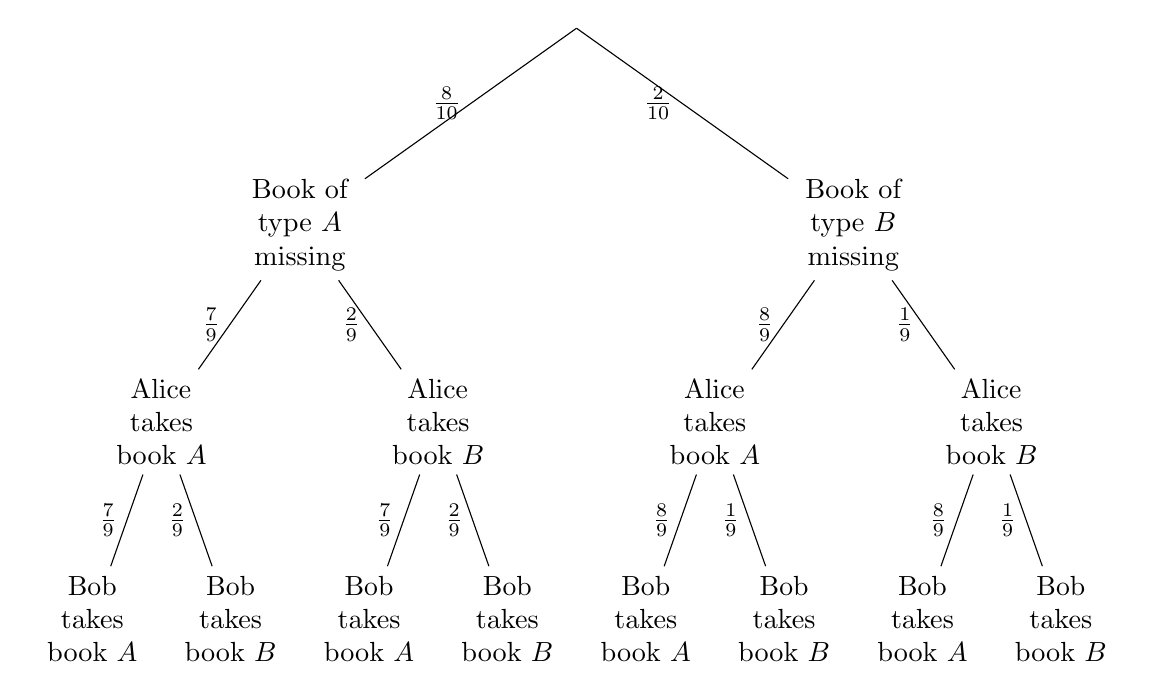
\begin{tikzpicture}[grow=down]%, sloped]
		\tikzstyle{node} = [text width=4em, text centered]
		\tikzstyle{prob} = [left]
		\tikzstyle{level 1}=[level distance=2.5cm, sibling distance=20em]
		\tikzstyle{level 2}=[level distance=2.5cm, sibling distance=10em]
		\tikzstyle{level 3}=[level distance=2.5cm, sibling distance=5em]
		important/.style={draw=red,line width=1.5pt,edge={red,line width=1.5pt,draw}},
		\coordinate
			child
			{
				node[node] {Book of type $A$ missing}
					child
					{
						node[node] {\A takes book $A$}
						child
						{
							node[node] {\B takes book $A$}
							edge from parent
							node[prob] {$\frac{7}{9}$}
						}
						child
						{
							node[node] {\B takes book $B$}
							edge from parent
							node[prob] {$\frac{2}{9}$}
						}
						edge from parent 
						node[prob] {$\frac{7}{9}$}
					}
					child
					{
						node[node] {\A takes book $B$}
						child
						{
							node[node] {\B takes book $A$}
							edge from parent
							node[prob] {$\frac{7}{9}$}
						}
						child
						{
							node[node] {\B takes book $B$}
							edge from parent
							node[prob] {$\frac{2}{9}$}
						}
						edge from parent 
						node[prob] {$\frac{2}{9}$}
					}
				edge from parent 
				node[prob] {$\frac{8}{10}$}
			}
			child
			{
				node[node] {Book of type $B$ missing}
					child
					{
						node[node] {\A takes book $A$}
						child
						{
							node[node] {\B takes book $A$}
							edge from parent
							node[prob] {$\frac{8}{9}$}
						}
						child
						{
							node[node] {\B takes book $B$}
							edge from parent
							node[prob] {$\frac{1}{9}$}
						}
						edge from parent 
						node[prob] {$\frac{8}{9}$}
					}
					child
					{
						node[node] {\A takes book $B$}
						child
						{
							node[node] {\B takes book $A$}
							edge from parent
							node[prob] {$\frac{8}{9}$}
						}
						child
						{
							node[node] {\B takes book $B$}
							edge from parent
							node[prob] {$\frac{1}{9}$}
						}
						edge from parent 
						node[prob] {$\frac{1}{9}$}
					}
				edge from parent 
				node[prob] {$\frac{2}{10}$}
			};
		\end{tikzpicture}
	\end{figure}
	\begin{align*}
		\prob(E) & = \left( \frac{8}{10} \right) \left( \frac{7}{9} \right) + \left( \frac{2}{10} \right) \left( \frac{8}{9} \right)                                                                                                                                                                                                                               \\
                         & = \frac{8}{10}                                                                                                                                                                                                                                                                                                                                  \\
		\prob(F) & = \left( \frac{2}{10} \right) \left( \frac{8}{9} \right) \left( \frac{8}{9} \right) + \left( \frac{2}{10} \right) \left( \frac{1}{9} \right) \left( \frac{8}{9} \right) + \left( \frac{8}{10} \right) \left( \frac{7}{9} \right) \left( \frac{7}{9} \right) + \left( \frac{8}{10} \right) \left( \frac{2}{9} \right) \left( \frac{7}{9} \right) \\
                         & = \frac{8}{10}
	\end{align*}
	Therefore,
	\begin{align*}
		\prob(E \cap F) & = \left( \frac{2}{10} \right) \left( \frac{8}{9} \right) \left( \frac{8}{9} \right) + \left( \frac{8}{10} \right) \left( \frac{7}{9} \right) \left( \frac{7}{9} \right) \\
                                & \neq \prob(E) \prob(F)
	\end{align*}<++>
	Therefore, the events are not independent.
\end{solution}

\begin{definition}
	Three events, $A$, $B$, and $C$, are said to be independent if
	\begin{align*}
		\prob(A \cap B \cap C) & = \prob(A) \prob(B) \prob(C) \\
		\prob(A \cap B)        & = \prob(A) \prob(B)          \\
		\prob(B \cap C)        & = \prob(B) \prob(C)          \\
		\prob(C \cap A)        & = \prob(C) \prob(A)
	\end{align*}
\end{definition}

\clearpage
\part{Random Variables}

\section{Discrete Random Variables}

\begin{definition}[Random variable]
	A function $X : \Omega \to \mathbb{R}$ which maps points from the sample space to the real line is called a random variable.
\end{definition}

\begin{question}
	Three balls are to be randomly selected, without replacement, from an urn containing $20$ balls numbered $1$ to $20$.
	If \A bets that at least one of the balls drawn has a number as large as or larger than $17$, what is the probability that \A wins the bet?
\end{question}

\begin{solution}
	Let $X$ be the largest number selected.\\
	Therefore, $X$ is a random variable which has a value from $\{3,\dots,20\}$.\\
	Let the value of the highest valued ball be $i$.
	Therefore, the number of ways to select the remaining two balls is $\comb{i - 1}{2}$.\\
	Therefore, the probability of the value of the highest valued ball being $i$ is
	\begin{align*}
		\prob(X = i) & = \frac{\comb{i - 1}{2}}{\comb{20}{3}}
	\end{align*}
	Therefore,
	\begin{align*}
		\prob(X \ge 17) & = \prob(X = 17) + \prob(X = 18) + \prob(X = 19) + \prob(X = 20) \\
                                & = \frac{\comb{16}{2} + \comb{17}{2} + \comb{18}{2} + \comb{19}{2}}{\comb{20}{3}}
	\end{align*}
\end{solution}

\section{Cumulative Distribution Function}

\begin{definition}[Cumulative distribution function]
	The function
	\begin{align*}
		F(x) & = \prob(X \le x)
	\end{align*}
	for $-\infty < x \le x$, is called the cumulative distribution function of the variable $X$.
\end{definition}

\begin{question}
	Let $X$ be the result of a die roll.
	Plot the cumulative distribution function of $X$.
\end{question}

\begin{solution}
	\begin{figure}[H]
		\centering
		\begin{tikzpicture}[scale = 1.5]
			\def\xMIN{-1};
			\def\xMAX{7};
			\def\yMIN{-1};
			\def\yMAX{2};

			\begin{scope}[stealth-stealth]
				\draw (\xMIN,0) -- (\xMAX,0) node [right] {$x$};
				\draw (0,\yMIN) -- (0,\yMAX) node [above] {$\cdf(X)$};
			\end{scope}

			\begin{scope}
				\draw (-\xMIN,0) -- (1,0);
				\draw (1,0) circle (1pt);
			\end{scope}

			\begin{scope}
				\begin{scope}
					\filldraw (1,1/6) circle (1pt);
					\draw (1,1/6) -- (2,1/6);
					\draw (2,1/6) circle (1pt);
				\end{scope}
				\begin{scope}
					\filldraw (2,2/6) circle (1pt);
					\draw (2,2/6) -- (3,2/6);
					\draw (3,2/6) circle (1pt);
				\end{scope}
				\begin{scope}
					\filldraw (3,3/6) circle (1pt);
					\draw (3,3/6) -- (4,3/6);
					\draw (4,3/6) circle (1pt);
				\end{scope}
				\begin{scope}
					\filldraw (4,4/6) circle (1pt);
					\draw (4,4/6) -- (5,4/6);
					\draw (5,4/6) circle (1pt);
				\end{scope}
				\begin{scope}
					\filldraw (5,5/6) circle (1pt);
					\draw (5,5/6) -- (6,5/6);
					\draw (6,5/6) circle (1pt);
				\end{scope}
				\begin{scope}
					\filldraw (6,6/6) circle (1pt);
					\draw (6,6/6) -- (\xMAX,6/6);
				\end{scope}
			\end{scope}
		\end{tikzpicture}
		\caption{Cumulative Distribution Function for a Die Roll}
		\label{fig:Cumulative_Distribution_Function_for_a_Die_Roll}
	\end{figure}
\end{solution}

\section{Probability Mass Function}

\begin{definition}[Discrete random variable]
	A random variable that can have at most a countable number of possible values is said to be discrete.
\end{definition}

\begin{definition}[Probability mass function]
	A function which gives the probability of a discrete random variable $X$ having value $x$ is called the probability mass function of $X$.
	It is denoted as $\prob(X = x)$.
\end{definition}

\begin{question}
	The probability mass function of a random variable $X$ is given by
	\begin{align*}
		\prob(X = i) & = \frac{c \lambda^i}{i!}
	\end{align*}
	where $i \in \mathbb{W}$, and $\lambda > 0$.\\
	Find
	\begin{enumerate}
		\item $\prob(X = 0)$
		\item $\prob(X > 2)$
	\end{enumerate}
\end{question}

\begin{solution}
	\begin{enumerate}[leftmargin=*]
		\item
			\begin{align*}
				\sum\limits_{i = 0}^{\infty} \prob(X = i)                      & = 1 \\
				\therefore \sum\limits_{i = 0}^{\infty} \frac{c \lambda^i}{i!} & = 1 \\
				\therefore c \sum\limits_{i = 0}^{\infty} \frac{\lambda^i}{i!} & = 1 \\
				\therefore c e^{\lambda}                                       & = 1 \\
				\therefore c                                                   & = e^{-\lambda}
			\end{align*}
			Therefore,
			\begin{align*}
				\prob(X = i) & = \frac{e^{-\lambda} \lambda^i}{i!}
			\end{align*}
			Therefore,
			\begin{align*}
				\prob(X = 0) & = \frac{e^{-\lambda} \lambda^0}{0!} \\
                                             & = e^{-\lambda}
			\end{align*}
		\item
			\begin{align*}
				\sum\limits_{i = 0}^{\infty} \prob(X = i)                      & = 1 \\
				\therefore \sum\limits_{i = 0}^{\infty} \frac{c \lambda^i}{i!} & = 1 \\
				\therefore c \sum\limits_{i = 0}^{\infty} \frac{\lambda^i}{i!} & = 1 \\
				\therefore c e^{\lambda}                                       & = 1 \\
				\therefore c                                                   & = e^{-\lambda}
			\end{align*}
			Therefore,
			\begin{align*}
				\prob(X = i) & = \frac{e^{-\lambda} \lambda^i}{i!}
			\end{align*}
			Therefore,
			\begin{align*}
				\prob(X > 2) & = 1 - \prob(X \le 2)                             \\
                                             & = 1 - \prob(X = 2) - \prob(X = 1) - \prob(X = 0) \\
                                             & = 1 - \frac{e^{-\lambda} \lambda^2}{2!} - \frac{e^{-\lambda} \lambda^1}{1!} - \frac{e^{-\lambda} \lambda^0}{0!}
			\end{align*}
	\end{enumerate}
\end{solution}

\begin{definition}
	If $X$ is a discrete random variable having a probability mass function $P(X = x)$, then the expectation or the expected value of $X$ is defined to be
	\begin{align*}
		\expct[X] & = \sum\limits_{\left\{ x | \prob(X = x) > 0 \right\}} x \prob(X = x)
	\end{align*}
\end{definition}

\begin{question}
	Find $\expct[X]$ where $X$ is the outcome of rolling a fair die.
\end{question}

\begin{solution}
	\begin{align*}
		\expct[x] & = \sum\limits_{x = 1}^{6} \frac{1}{6} x \\
                          & = 3.5
	\end{align*}
\end{solution}

\begin{question}
	A class of $120$ students is driven in $3$ buses to a symphonic perfomance.
	There are $36$ students in the first bus, $14$ in the second, and $44$ in the third bus.
	When the buses arrive, a student is randomly chosen.
	Let $X$ denote the number of students on the bus of the chosen student.
	Find $\expct[X]$.
\end{question}

\begin{solution}
	\begin{align*}
		\prob(X = 36) & = \frac{36}{120} \\
		\prob(X = 40) & = \frac{40}{120} \\
		\prob(X = 44) & = \frac{44}{120}
	\end{align*}
	Therefore,
	\begin{align*}
		\expct[X] & = 36 \left( \frac{36}{120} \right) + 40 \left( \frac{40}{120} \right) + 44 \left( \frac{44}{120} \right) \\
                          & = 40.2667
	\end{align*}
\end{solution}

\begin{question}
	$X$ has the following distribution.
	\begin{align*}
		\prob(X = -1) & = 0.2 \\
		\prob(X = 0)  & = 0.5 \\
		\prob(X = 1)  & = 0.3
	\end{align*}
	Find $\expct\left[ x^2 \right]$.
\end{question}

\begin{solution}
	Let
	\begin{align*}
		Y & = X^2
	\end{align*}
	Therefore,
	\begin{align*}
		\prob(Y = 0) & = \prob(X = 0)                 \\
                             & = 0.5                          \\
		\prob(Y = 1) & = \prob(X = -1) + \prob(X = 1) \\
                             & = 0.5
	\end{align*}
	Therefore,
	\begin{align*}
		\expct[Y] & = \expct\left[ X^2 \right] \\
                          & = (0) (0.5) + (1) (0.5)    \\
                          & = 0.5
	\end{align*}
\end{solution}

\begin{theorem}
	If $X$ is a discrete random variable that takes on one of the values $x_i$, where $i \in \mathbb{N}$, with probability mass function $\prob(X = x_i)$.
	Then, for any real valued function $g$,
	\begin{align*}
		\expct\left[ g(x) \right] & = \sum\limits_{i} g(x_i) \prob(x = x_i)
	\end{align*}
\end{theorem}

\begin{question}
	A product that is sold seasonally yeilds a net profit of $b$ for each unit sold and a net loss of $l$ for each unit left unsold when the season ends.
	The number of units of the product that are sold at a specific store during any season is a random variable $X$, with probability mass function such that
	\begin{align*}
		\prob(X = i) & = \prob(i)
	\end{align*}
	where $i \in \mathbb{N}$.
	If the store must stock this product in advance, determine the number of units the store should stock, so as to maximize its profit.
\end{question}

\begin{solution}
	Let the number of units sold by $X$.\\
	Let the number of units stocked by $s$.\\
	Therefore, the total profit is
	\begin{align*}
		\pi(s) &=
			\begin{cases}
				b X - (s - X) l & ;\quad X \le s \\
				b s             & ;\quad X > s   \\
			\end{cases}
	\end{align*}
	Therefore,
	\begin{align*}
		\expct\left[ \pi(s) \right] & = \sum\limits_{i = 0}^{s} \left( b i - (s - i) l \right) \prob(X = i) + \sum\limits_{i = s + 1}^{\infty} s b \prob(X = i)                                 \\
                                            & = (b + l) \sum\limits_{i = 0}^{s} i \prob(X = i) - s l \sum\limits_{i = 0}^{s} \prob(X = i) + s b \left( 1 - \sum\limits_{i = 0}^{s} \prob(X = i) \right) \\
                                            & = (b + l) \sum\limits_{i = 0}^{s} i \prob(X = i) - (b + l) s \sum\limits_{i = 0}^{s} \prob(X = i) + s b                                                   \\
                                            & = s b + (b + l) \sum\limits_{i = 0}^{s} (i - s) \prob(X = i)
	\end{align*}
	Therefore,
	\begin{align*}
		\expct\left[ \pi(s + 1) \right] & = b (s + 1) + (b + l) \sum\limits_{i = 0}^{s + 1} (i - s - 1) \prob(X = i) \\
                                                & = b (s + 1) + (b + l) \sum\limits_{i = 0}^{s} (i - s - 1) \prob(X = i)     \\
	\end{align*}
	Therefore,
	\begin{align*}
		\expct\left[ \pi(s + 1) \right] - \expct\left[ \pi(s) \right] & = b - (b + l) \sum\limits_{i = 0}^{s} \prob(X = i)
	\end{align*}
	Therefore, increasing the stock is profitable when
	\begin{align*}
		\sum\limits_{i = 0}^{s} \prob(X = i) & < \frac{b}{b + l}
	\end{align*}
\end{solution}

\section{Variance}

\begin{definition}[Variance]
	The variance of a random variable $X$ is defined to be
	\begin{align*}
		\var(x) & = \expct\left[ \left( X - \expct[X] \right)^2 \right] \\
                        & = \expct\left[ X^2 \right] - \expct[X]^2
	\end{align*}
\end{definition}

\begin{question}
	Calculate $\var(X)$ where $X$ represents the outcome of rolling a fair die.
\end{question}

\begin{solution}
	\begin{align*}
		\expct[X]                & = \sum\limits_{x = 1}^{6} \frac{1}{6} x   \\
                                         & = \frac{7}{2}                             \\
		\expct\left[ X^2 \right] & = \sum\limits_{x = 1}^{6} \frac{1}{6} x^2 \\
                                         & = \frac{91}{6}
	\end{align*}
	Therefore,
	\begin{align*}
		\var(X) & = \expct\left[ X^2 \right] - \expct[X]^2 \\
                        & = \frac{91}{6} - \frac{49}{4}            \\
                        & = \frac{35}{12}
	\end{align*}
\end{solution}

\begin{theorem}
	\begin{align*}
		\var(a X + b) & = a^2 \var(X)
	\end{align*}
\end{theorem}

\begin{proof}
	\begin{align*}
		\var(a X + b) & = \expct\left[ \left( a X + b - \expct[a X + b] \right)^2 \right] \\
                              & = \expct\left[ \left( a X + b - a \expct[X] - b \right)^2 \right] \\
                              & = \expct\left[ a^2 \left( X - \expct[X] \right)^2 \right]         \\
                              & = a^2 \expct\left[ \left( x - \expct[x] \right)^2 \right]         \\
                              & = a^2 \var(x)
	\end{align*}
\end{proof}

\begin{question}
	You have a coin with probability $p$ of getting `Heads'.
	You flip this coin twice.\\
	For each flip, if the result is `Heads', you win $\$30$.
	If the result is `Tails', you lose $\$20$.\\
	Let $X$ be your profit in the game.
	\begin{enumerate}
		\item What is the sample space?
		\item Describe the probability mass function of $X$.
		\item Describe the cumulative distribution function of $X$.
		\item What is the expected value of $X$?
		\item What is the value of $p$ upto which you would agree to participate in the game?
		\item What is $\var(X)$?
		\item What is $\sd(X)$?
	\end{enumerate}
\end{question}

\begin{solution}
	\begin{enumerate}[leftmargin=*]
		\item
			\begin{align*}
				S & = \left\{ (30 + 30) , (30 - 20) , (-20 - 20) \right\} \\
                                  & = \left\{ 60 , 10 , -40 \right\}
			\end{align*}
		\item
			\begin{align*}
				\prob(X = x) &=
					\begin{cases}
						p^2         & ;\quad x = 60  \\
						2 p (1 - p) & ;\quad x = 10  \\
						(1 - p)^2   & ;\quad x = -40 \\
					\end{cases}
			\end{align*}
		\item
			\begin{align*}
				\cdf(X) &=
					\begin{cases}
						0                             & ;\quad x < -40        \\
						(1 - p)^2                     & ;\quad -40 \le x < 10 \\
						(1 - p)^2 + 2 p (1 - p)       & ;\quad 10 \le x < 60  \\
						(1 - p)^2 + 2 p (1 - p) + p^2 & ;\quad x \le 60       \\
					\end{cases}
			\end{align*}
		\item
			\begin{align*}
				\expct[X] & = (-40) (1 - p)^2 + (10) \left( 2 p (1 - p) \right) + (60) \left( p^2 \right) \\
                                          & = 100p - 40
			\end{align*}
		\item
			The game should be played as long as the expected value of $X$ is non negative.\\
			Therefore,
			\begin{align*}
				\expct[X]             & \ge 0 \\
				\therefore 100 p - 40 & \ge 0 \\
				\therefore p          & \ge 0.4
			\end{align*}
		\item
			\begin{align*}
				\expct\left[ x^2 \right] & = (-40)^2 (1 - p)^2 + (10)^2 2 p (1 - p) + (60)^2 p^2 \\
                                                         & = 5000 p^2 - 3000 p + 1600                            \\
				\expct[x]^2              & = (100 p - 40)^2                                      \\
                                                         & = 10000 p^2 - 8000 p + 1600
			\end{align*}
			Therefore,
			\begin{align*}
				\var(X) & = \expct\left[ X^2 \right] - \expct[X]^2 \\
                                        & = 5000 p (1 - p)
			\end{align*}
		\item
			\begin{align*}
				\sd(X) & = \sqrt{\var(X)} \\
                                       & = \sqrt{5000 p (1 - p)}
			\end{align*}
	\end{enumerate}
\end{solution}

\clearpage
\part{Special Distributions}

\section{Bernoulli and Binomial Random Variables}

\begin{definition}[Bernoulli random variable]
	A random variable $X$ is said to be a Bernoulli random variable if its probability mass function is given by
	\begin{align*}
		\prob(X = 0) & = 1 - p \\
		\prob(X = 1) & = p
	\end{align*}
\end{definition}

\begin{theorem}
	For a Bernoulli random variable,
	\begin{align*}
		\expct[x] & = p \\
		\var(x)   & = p (1 - p)
	\end{align*}
\end{theorem}

\begin{definition}[Binomial random variable]
	Consider $n$ independent trials, each of which has a probability of success $p$, and probability of failure $1 - p$.
	If $X$ represents the number of successes that occur in the $n$ trials, then $X$ is said to be a binomial random variable with parameters $(n,p)$.
	It is denoted as
	\begin{align*}
		X & \sim \bin(n,p)
	\end{align*}
\end{definition}

\begin{theorem}
	For a binomial random variable,
	\begin{align*}
		X & \sim \bin(n,p)
	\end{align*}
	the probability mass function is
	\begin{align*}
		\prob(X = i) & = \comb{n}{i} p^i (1 - p)^{n - i}
	\end{align*}
\end{theorem}

\begin{question}
	A die is rolled $5$ times.
	What is the probability that the result is $6$, $3$ times?
\end{question}

\begin{solution}
	Let $X$ be the number of times $6$ appears.\\
	Therefore,
	\begin{align*}
		X &\sim \bin\left( 5,\frac{1}{6} \right)
	\end{align*}
	Therefore,
	\begin{align*}
		\prob(X = i)            & = \comb{n}{i} p^i (1 - p)^{n - i} \\
		\therefore \prob(X = 3) & = \comb{5}{3} \left( \frac{1}{6} \right)^3 \left( \frac{5}{6} \right)^3
	\end{align*}
\end{solution}

\end{document}
